\chapter{Multi-task learning for extrapolation}
\label{chapMultiTaskExtrapolation}
In the current part we are interested in learning relationships in presence of multiple outputs, or learning an unknown functional relationship between an input space $X \in \mathbb{R}^{D_{inputs}}$ and outputs  $X \in \mathbb{R}^{D_{outputs}}$ ($D_{outputs}>1$). Performing regression on multiple-outputs can be split into two categories, firstly when we wish to discover relationships across several outputs, and secondly when we wish to enforce a known relationship between outputs as a bias into our learning algorithm.

When no information is between dependent outputs, we are interested in learning their interaction properties. This is setting also called as `multi-task learning' in machine learning literature. Several real world problems often exhibit strong correlations between many output variables, for example correlations across spatial coordinates ($x, y, z$) in an experiment. Learning relationships across outputs can improve the efficiency and prediction accuracy for the models, when compared to training the models separately \cite{caruana1998multitask}. These types of models are commonly called as Cokriging in Geostatistics \cite{helterbrand1994universal, chilès1999geostatistics, ver1998constructing}, or multi-task GP in machine learning \cite{alvarez2011kernels, bonilla_multi-task_2008, Boyle05dependentgaussian}.

When a relationship is known between outputs, enforcing such a relationship in a learning algorithm will mean that we have implemented a correct bias. Several types of relationships are exist in engineering design problems between outputs. The outputs can be results from multi-fidelity computer codes \cite{kennedy2000predicting, forrester2007multi, le2013multi}. The outputs can be related through a known equation, for example if we know that $acceleration = d(velocity)/d(time)$ and we measure both velocity and acceleration how to enforce the known equation into our model \cite{ginsbourger2013invariances, sarkka2011linear}. The outputs can be related through a known computer code, for example stress and forces in a known CSM code \cite{Constantinescu2013}. 

We split the part \ref{partIncorporateMultipleOutputs} of this thesis into two chapters. The current chapter (chapter \ref{chapMultiTaskExtrapolation})will describe the basics of cokriging/multi-task learning GP, present the cokriging interpolation model for outputs from a series of multi-fidelity simulations, and then propose a method to extrapolation high-fidelity simulations in presence of low-fidelity simulations. The next chapter \ref{chapAddingEquationsInGP} will describe how to encode known relationships between outputs, the most common form of this model is called as Gradient Enhanced Kriging (GEK) in the literature. Chapter \ref{chapAddingEquationsInGP} describes a more general class of these models, these can enable us to perform integral enhanced kriging, quadratic enhanced kriging or any functional relationship across outputs kriging. 

The current chapter unfolds as follows, section \ref{secMTGP} describes the various methods available in literature to perform Multi-Task GP (MTGP). Section \ref{secMultiFidelityMTGP} describes multi-task GP model in presence of outputs from different fidelitys, we also compare a normal MTGP with multi-fidelity GP. Section \ref{secMTGPExtrapolation} describes our model of extrapolation in MTGP. This chapter is influenced from the works of \cite{forrester2007multi, alvarez2011kernels, bonilla_multi-task_2008, Boyle05dependentgaussian, kennedy2000predicting, le2013multi}.

\section{Multi-task Gaussian Process}\label{secMTGP}
Suppose we have a \(D_{inputs}\) dimensional input space and a \(D_{outputs}\) (\(D_{outputs} > 1\) ) dimensional output space. Such that \(\{(x_{i}^{j}, y_{i}^{j})\}\) for \(i \in [1; N_{j}]\) are the training datasets for the \(j^{th}\) output. Here \(N_{j}\) is the number of measurement points for the \(j^{th}\) output, while \(x_{i}^{j} \in \mathbb{R}^{D_{inputs}}\) and \(y_{i}^{j} \in \mathbb{R}\). We next define \(x^{j} = \{x_{1}^{j}; x_{2}^{j}; \ldots ; x_{N_{j}}^{j}\}\) and \(y^{j} = \{y_{1}^{j}; y_{2}^{j}; \ldots ; y_{N_{j}}^{j}\}\) as the full matrices containing all the training points for the \(j^{th}\) output such that \(x^{j} \in \mathbb{R}^{N_{j} \times D_{inputs}}\) and \(y^{j} \in \mathbb{R}^{N_{j}}\). If \(\Sigma N_{j} = N\) for \(i \in [1, D]\). Hence \(N\) represents the total number of training points for all the outputs combined

\subsection{An extra dimension}\label{subsecAnExtraDimension}
One simple way of building joint model for multiple outputs is by treating them as a single-output GP but with extra dimension of the input dimension (equation \ref{eqMTGPDimension}) \cite{osborne2010bayesian}. 

\begin{equation}\label{eqMTGPDimension}
    y^{j}(x_{i}^{j}) = y_{full}(x_{i}^{j}, j)
\end{equation}

Henceforth we define the joint output vector \(y_{full} = [y^{1}; y^{2}; \ldots; y^{D_{outputs}}]\) such that all the output values are stacked one after the other, while \(Y \in \mathbb{R}^{N}\). Similarly, we define the joint input matrix as \(x_{full} = [x^{1}, 1; x^{2}, 2; x^{3}, 3, \ldots, x^{D_{outputs}, D_{outputs}}]\), having one extra dimension representing the output number, such that \(X \in \mathbb{R}^{N \times (D_{inputs}+1)}\). We can define a zero mean GP for the full set of inputs and outputs $\{x_{full}, y_{full}\}$, as equation \ref{eq:mogpJointPrior}.

\begin{equation}\label{eq:mogpJointPrior}
\begin{aligned}
       \Pr[y_{full}(x_{full})] & = \Pr\begin{bmatrix}   y_{full}(x^{1}, 1) \\ y_{full}(x^{2}, 2)   \end{bmatrix} \\
& = GP\begin{bmatrix}
   \begin{pmatrix}
   0\\ 
   0
   \end{pmatrix} ,& 
   \begin{pmatrix}
    Cov(y_{full}(x^{1}, 1), y_{full}(x^{1}, 1))  & Cov(y_{full}(x^{1}, 1), y_{full}(x^{2}, 2))\\ 
    Cov(y_{full}(x^{2}, 2), y_{full}(x^{1}, 1))     & Cov(y_{full}(x^{2}, 2), y_{full}(x^{2}, 2))
   \end{pmatrix}
   \end{bmatrix} \\
       & = GP(0, \myMatrix(K_{XX}))
\end{aligned}
   \end{equation}

We will denote the full joint covariance function as $K_{XX}$ (equation \ref{eqJointCovariance}). Since the a multi-output GP can be represented as a single output GP with an extra dimension, we can use all the kernel making techniques discussed in section \ref{secMultiDimensionalKernels} to current problem. 

\subsection{Simple Multi-task kernel}\label{simpleMultiTask}
\cite{bonilla2007multi} propose a simple model by multiplying the kernel on inputs with a kernel of extra dimension \ref{eqBonillaMTGP}.

\begin{align}\label{eqBonillaMTGP}
    Cov(Y(x_{1}, a), Y(x_{2}, b)) = \FUNC{k_{output}}(a, b) \times \FUNC{k_{input}}(x_{1}, x_{2})
\end{align}

There exists one issue though, the extra dimension is a categorical variable and has no measure of distance, i.e. the difference between two output numbers $a$ and $b$ is not defined. \cite{bonilla2007multi} define the covariance across outputs as equation \ref{eqKOutput}, this makes the matrix $k_{output}(a, b)$ positive definite and hence a valid kernel.

\begin{equation}\label{eqKOutput}
k_{output}(a, b) = LL^T
\end{equation}

The hyper-parameters of this equation are, hyper-parameters of the input covariance ($k_{input}(x_{1}^{a}, x_{2}^{b})$), and values of the lower triangular matrix $L$. When $k_{output}(a, b)$ is a diagonal matrix there is no cross-covariance across outputs, this implies that the outputs are independent of each other. In such a kernel design there is no transfer of information between outputs \cite{bonilla2007multi, o1998markov}, for a detailed derivation refer to appendix \textbf{give reference to appropriate appendix}.

We can write the Gram matrix for this simple function as equation \ref{eqGramMatrixSimpleMultiTask}.

\begin{equation}\label{eqGramMatrixSimpleMultiTask}
   \MAT{K_{XX}} =  \begin{bmatrix} k_{output}(1, 1) \odot \myMatrix{K}_{input}(x^{1}, x^{1}) & 
k_{output}(1, 2) \odot \myMatrix{K}_{input}(x^{1}, x^{2}) \\ 
k_{output}(2, 1) \odot \myMatrix{K}_{input}(x^{2}, x^{1}) &
k_{output}(2, 2) \odot \myMatrix{K}_{input}(x^{2}, x^{2}) 
\end{bmatrix}
\end{equation}

Figure \ref{subFigdrawsBonillaKernel} is a joint draws from such a kernel function between outputs $y^{1}$ and $y^{2}$. The matrix $k_{output} = [4, 0.2; 0.2, 1]$ while the covariance function between inputs $\FUNC{k_{input}}(x_{1}, x_{2})$ is a SE kernel with hyper-parameters $(\theta = [1, 0.2])$. We can observe that the variance of output $y^{1}$ is twice that of output $y^{2}$, this is because $\sqrt{k_{output}(1, 1)/k_{output}(2, 2)} = 2$.

\subsection{Linear Model of Coregionalization}\label{subsecLMC}
The next method considers the output variables as a linear combination of independent latent Gaussian Processes. It is called the Linear Model of Coregionalization in kriging literature \cite{goovaerts1997geostatistics} or Semiparametric Latent Factor Model in MTGP literature \cite{seeger2005semiparametric}. 

Suppose we have a set of $T$ latent GPs $U(x) = \{u^{1}(x), u^2(x), \ldots, u^{T}(x)\}$, where $u^{i}(x)$ is a GP with covariance $k_{u}^{i}(x_{1}, x_{2})$. Any linear combination of $u^{i}(x) \forall i \in T$ is a viable GP (section \ref{subsecStructureKernelsAddingKernels}), therefore we can define the GP of output $y^{j}$ as equation \ref{eqLinearCombo}. 

\begin{equation}\label{eqLinearCombo}
y^{j}(x) = \sum_{i=1}^{T} \alpha^{ij}u^{i}(x)
\end{equation}

The covariance function can thus be written as equation \ref{eqLMC}.

\begin{equation} 
 \begin{aligned}
Cov(Y(x_{1}, a), Y(x_{2}, b)) & = Cov(\sum_{i=1}^{T} \alpha^{ia}u^{i}(x_{1}), \sum_{i=1}^{T} \alpha^{ib}u^{i}(x_{2})) \\ 
& = \sum_{i=1}^{T} \alpha^{ia}\alpha^{ib} Cov(u^{i}(x_{1}), u^{i}(x_{2})) \\ 
& = \sum_{i=1}^{T} \alpha^{ia}\alpha^{ib}k_{u}^{i}(x_{1}, x_{2}) \\ 
& = \sum_{i=1}^{T} k_{output}^{i}(a, b) \times k_{u}^{i}(x_{1}, x_{2})
 \end{aligned}
\end{equation}

The covariance between the output dimension $k_{output}^{i}$ is also called the coregionalization matrix, and is of size $D_{outputs} \times D_{outputs}$. It can be written as equation \ref{eqCovarianceAcrossOutputs}, making it a positive definite matrix.

\begin{equation}\label{eqCovarianceAcrossOutputs}
k_{output}^{i} = \begin{bmatrix}
\alpha^{i1}\\ 
\alpha^{i2}\\ 
\vdots\\ 
\alpha^{iT}
\end{bmatrix} \times \begin{bmatrix}
\alpha^{i1} & \alpha^{i2} & \ldots & \alpha^{iT}
\end{bmatrix}
\end{equation}

Note, when $T = 1$ and $D_{outputs} > 1$ the Linear Model of Coregionalization is equivalent to the model proposed by \cite{bonilla2007multi}. While, when $T > 1$ and $D_{outputs} = 1$ the Linear Model of Coregionalization model resembles an additive covariance of $T$ individual covariances.

\textbf{Check again}
Figure \ref{subFigdrawsLCMKernel} shows 3 joint draws from a `Linear Model of Coregionalization' kernel function between outputs $y^{1}$ and $y^{2}$. We use two latent functions for figure; the kernels between output dimensions are $k_{output}^{1} = [4, 0.2; 0.2, 1]$ and $k_{output}^{2} = [1, 0.2; 0.2, 1]$, while the covariance function between inputs are SE kernel with hyper-parameters $(\theta = [1, 0.2])$ for the first latent process and $(\theta = [1, 0.1])$ for the second latent process. The length-scale of the functions is determined by the smallest length-scale of the latent processes.

\begin{figure}[!ht]
  \centering
    \subfigure[{Joint draws from such a simple multi-task kernel function between outputs $y^{1}$ and $y^{2}$. The matrix $k_{output} = [4, 0.2; 0.2, 1]$ while the covariance function between inputs $\FUNC{k_{input}}(x_{1}, x_{2})$ is a SE kernel with hyper-parameters $(\theta = [1, 0.2])$. We can observe that the variance of output $y^{1}$ is twice that of output $y^{2}$, this is because $\sqrt{k_{output}(1, 1)/k_{output}(2, 2)} = 2$.}]
  {
        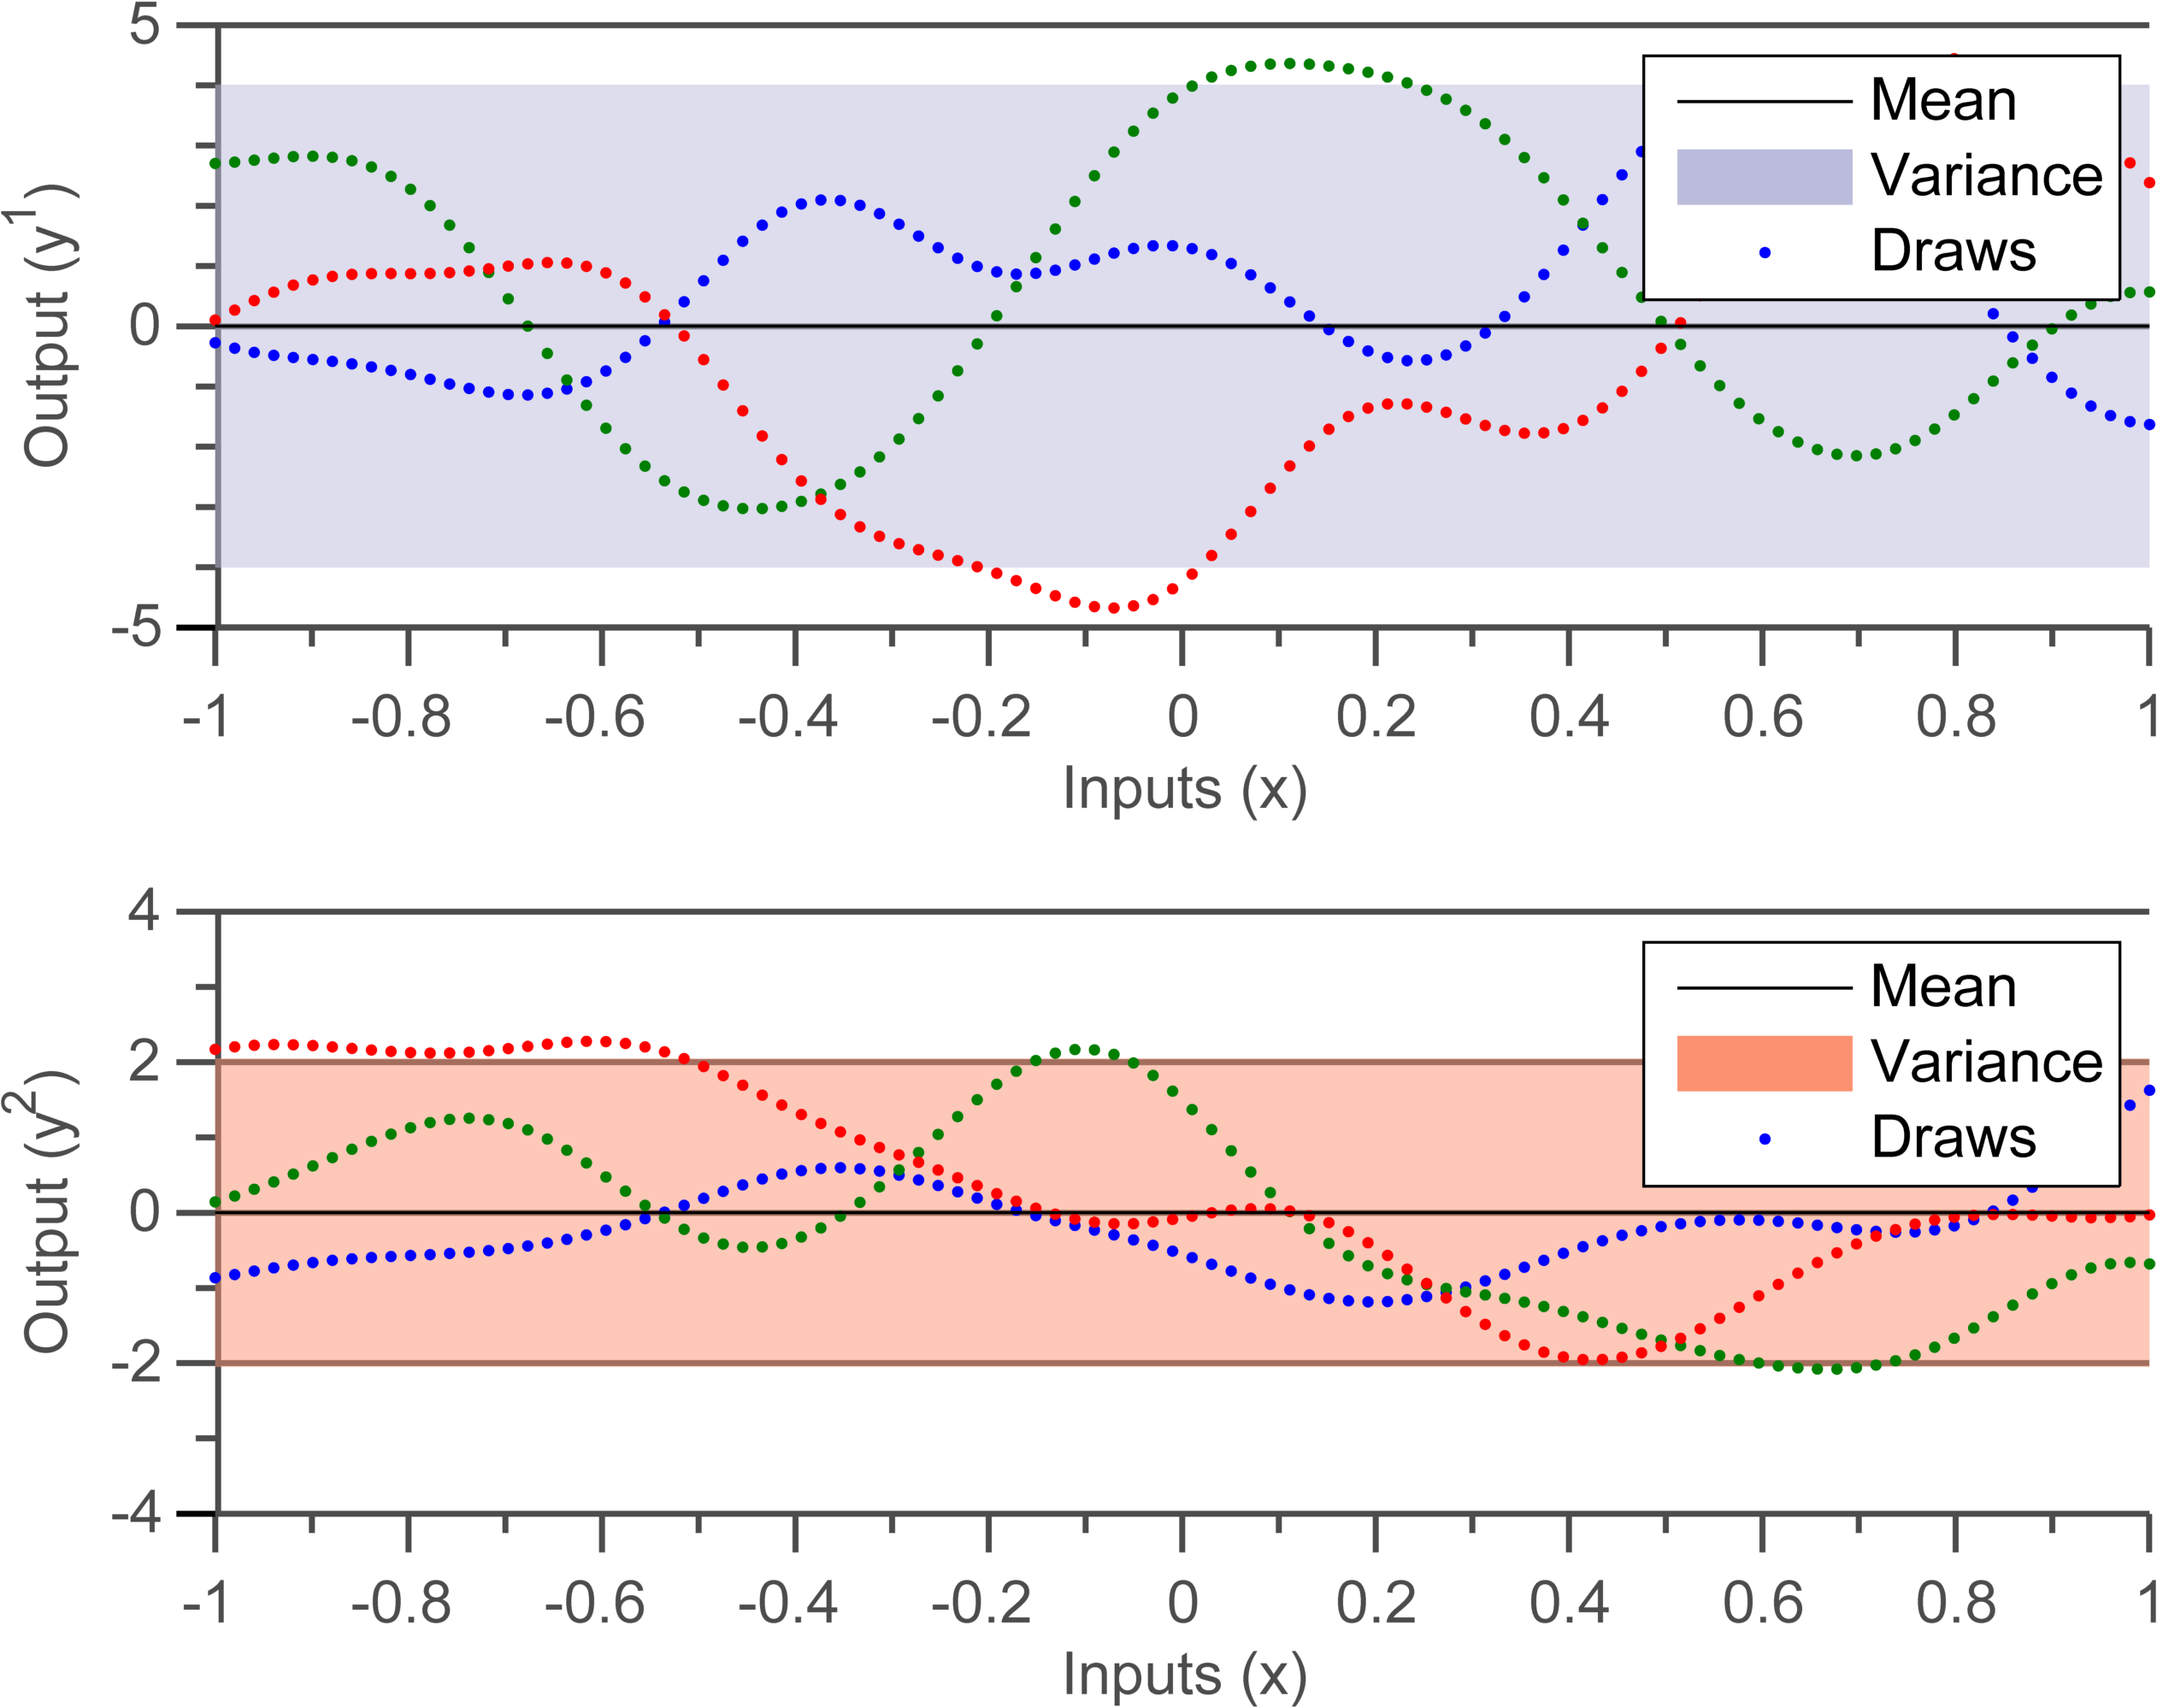
\includegraphics[width=0.45\textwidth]
        {images/part3/drawsBonillaKernel}
        \label{subFigdrawsBonillaKernel}
  }\quad
\subfigure[{Joint draws from a `Linear Model of Coregionalization' kernel function between outputs $y^{1}$ and $y^{2}$. We use two latent functions for figure; the kernels between output dimensions are $k_{output}^{1} = [4, 0.2; 0.2, 1]$ and $k_{output}^{2} = [1, 0.2; 0.2, 1]$, while the covariance function between inputs are SE kernel with hyper-parameters $(\theta = [1, 0.2])$ for the first latent process and $(\theta = [1, 0.1])$ for the second latent process. The length-scale of the functions is determined by the smallest length-scale of the latent processes.}]
  {
        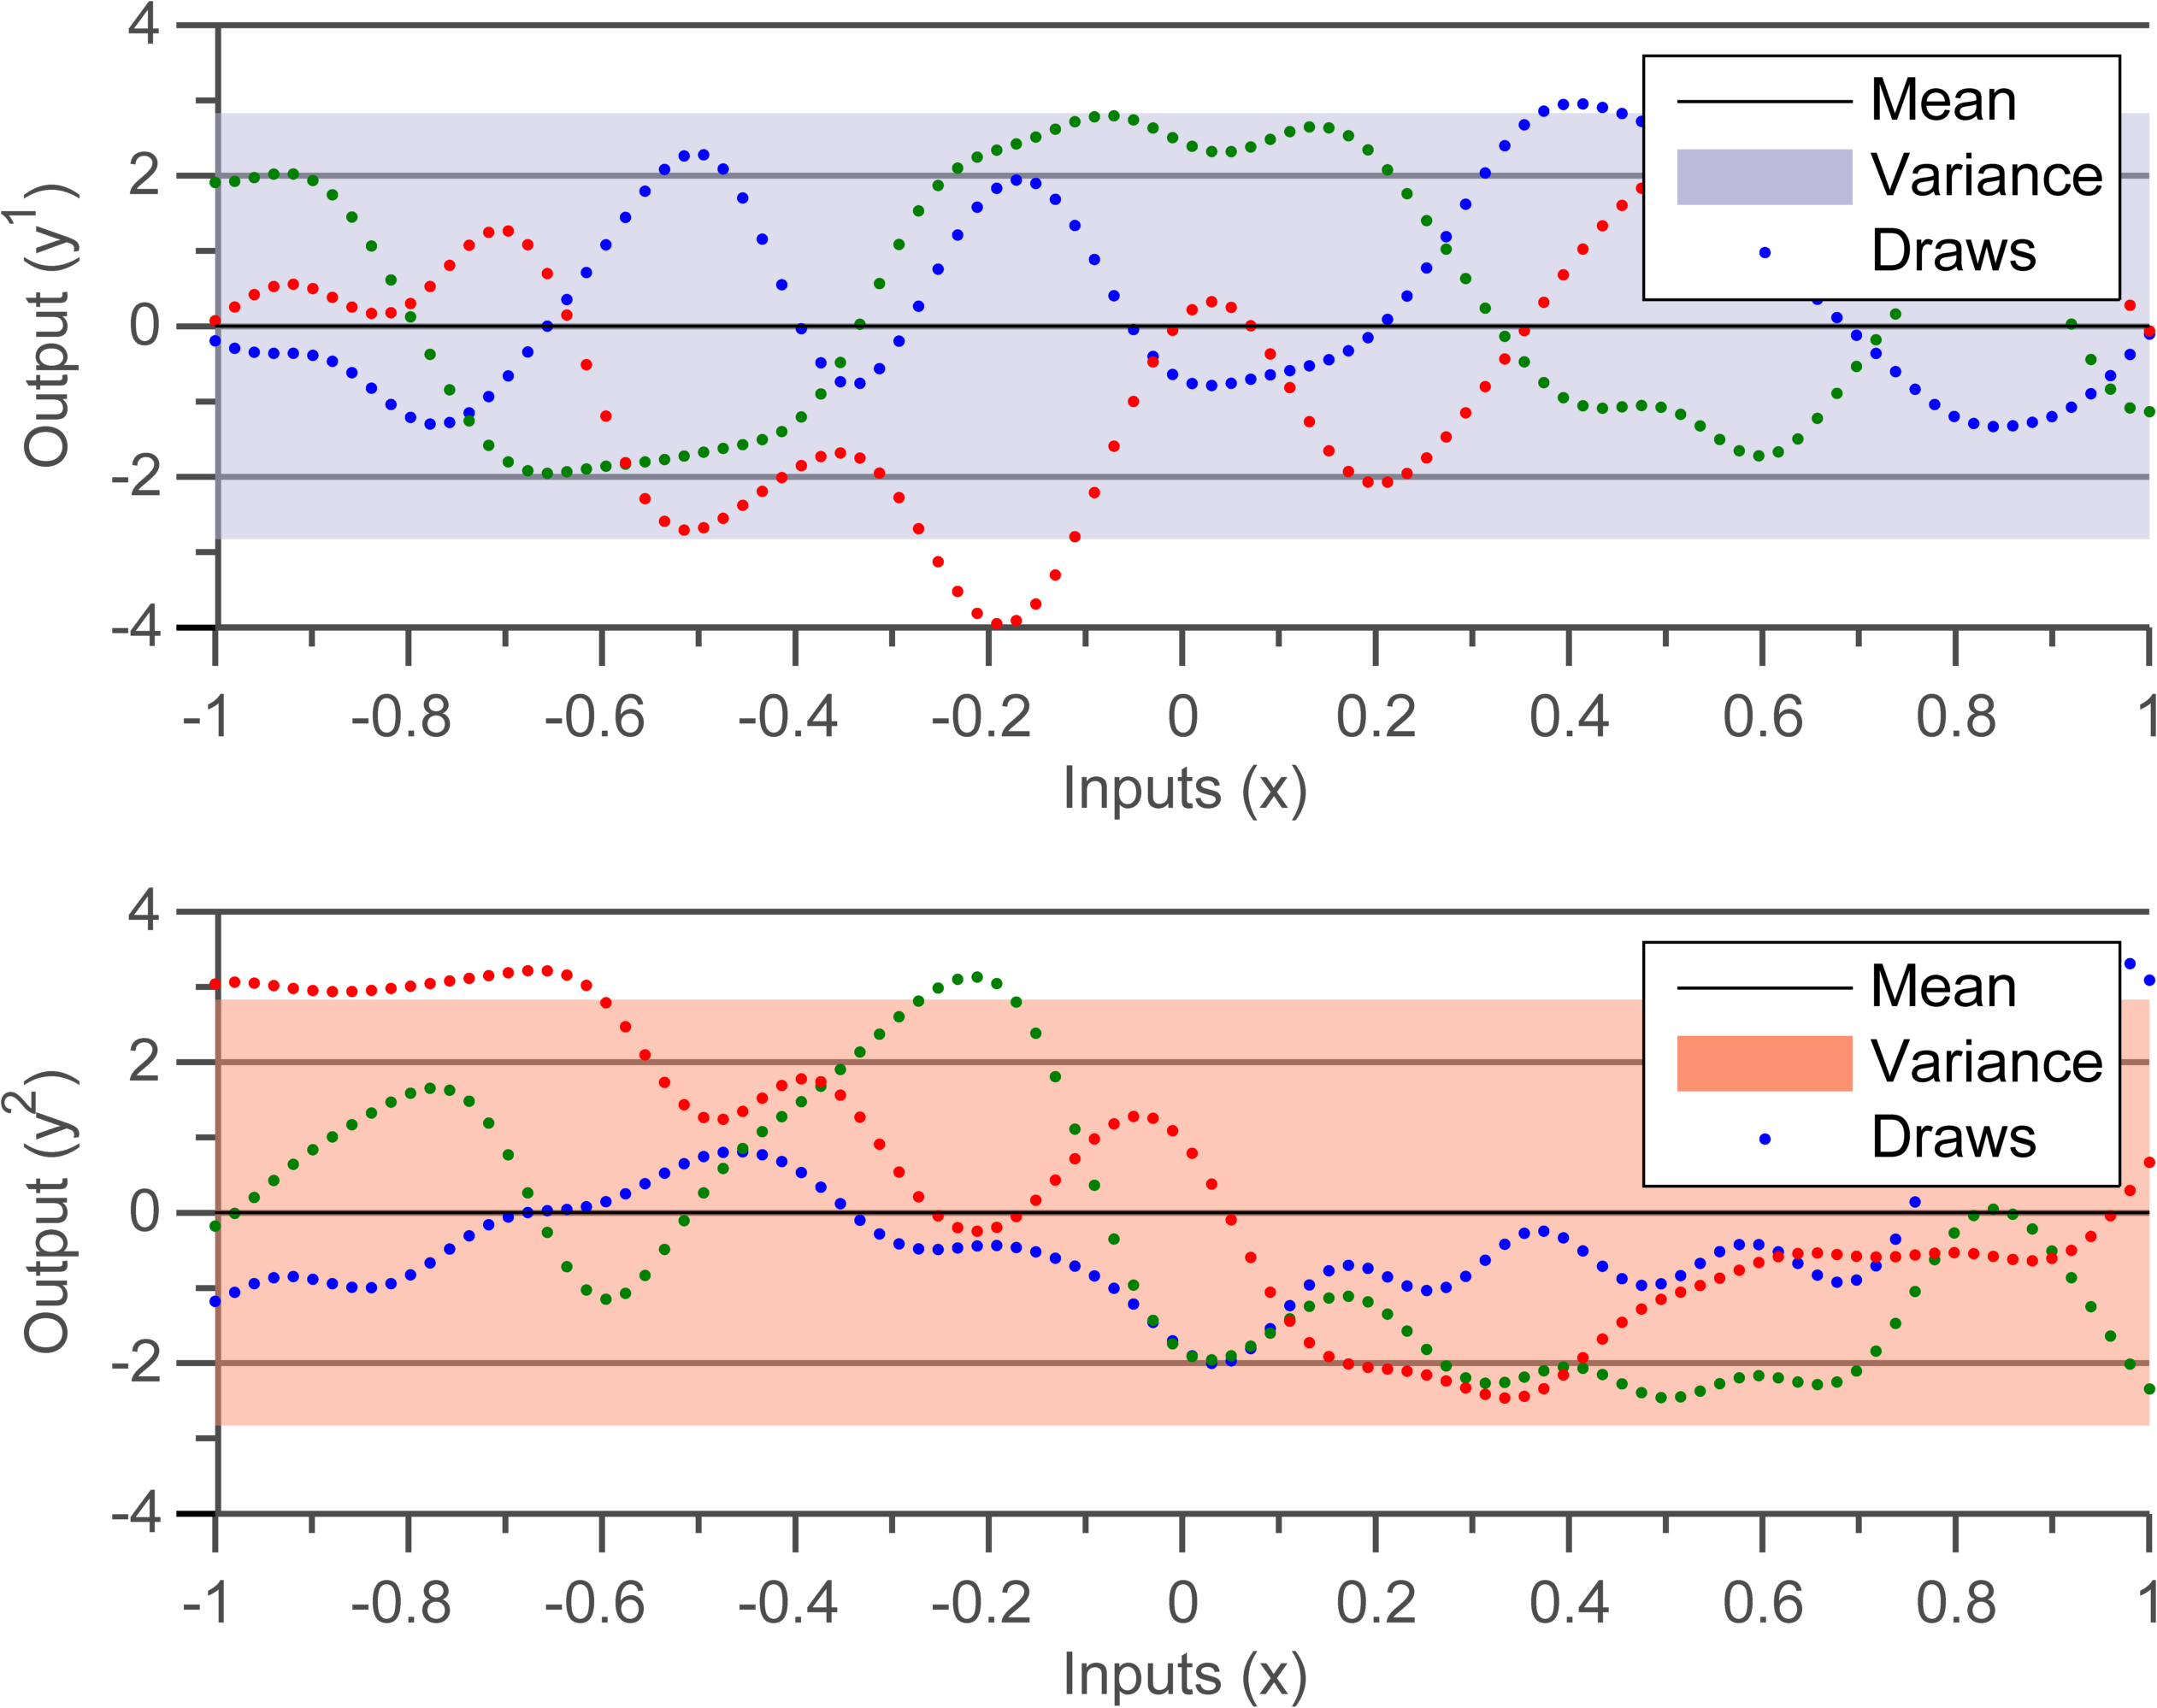
\includegraphics[width=0.45\textwidth]
        {images/part3/drawsLCMKernel}
        \label{subFigdrawsLCMKernel}
  }\quad

       \caption{Joint draws defined by multi-task priors: the solid black line defines the mean function, shaded blue region defines 95\% confidence interval (2$\sigma$) distance away from the mean. The dashed lines represent five functions drawn at random from a GP prior. We can observe that figure \ref{subFigdrawsLCMKernel} varies faster when compared to figure \ref{subFigdrawsBonillaKernel} due to smaller length scale hyper-parameter in one of the latent functions.       }
       \label{figJointPriors}
\end{figure}

\subsection{Convoluted Gaussian Process}\label{subsecConvolutedGP}
The next extension to creating MTGP covariances is assuming that outputs are generated from a convolution of latent GPs \cite{higdon2002space, Boyle05dependentgaussian}. First and second order
differential equations, as well as partial differential equations, can be accommodated in a covariance function using this method \cite{journals/jmlr/AlvarezLL09}.

Suppose we have a set of $T$ latent GPs $U(x) = \{u^{1}(x), u^2(x), \ldots, u^{T}(x)\}$, where $u^{i}(x)$ is a GP with covariance $k_{u}^{i}(x_{1}, x_{2})$. A convolution of $u^{i}(x) \forall i \in T$ using a smoothing function $h^{ij}(x)$ is a viable GP (section \ref{subsecStructureKernelsAddingKernels}), (equation \ref{eqConvolutionCombo}).

\begin{equation}\label{eqConvolutionCombo}
y^{j}(x) = \sum_{i=1}^{T} \int h^{ij}(x - z) u^{i}(z) dz
\end{equation}

The covariance can thus be written as:

\begin{equation} \label{eqConvolutionCovariance}
 \begin{aligned}
Cov(Y(x_{1}, a), Y(x_{2}, b)) & = \sum_{i=1}^{T} \int h^{ia}(x_{1} - z) \int h^{ib}(x_{2} - z') k_{u}^{i}(z, z') dz dz'
 \end{aligned}
\end{equation}

\cite{Boyle05dependentgaussian} define the latent GPs $u^{i}(x)$ as a set of white noise Gaussians. When the smoothing function is a Kronecker delta function ($h^{ij}(x) = \alpha^{ij}\delta(x)$), then the MTGP defined through a convolution process becomes a Linear Model of Coregionalization. \cite{journals/jmlr/AlvarezLL09} use the above kernels to solve differential equations, the smoothing function $h^{ij}(x)$ is the Green's function of the differential equation for their case.  

\subsection{Multi-fidelity Cokriging}\label{secMultiFidelityMTGP}
One of the first multi-fidelity model was based on a linear regression formulation \cite{craig1998constructing, goldstein2007bayes}. Since kriging is better method to perform regression when compared to Linear regression, the multi-fidelity model was improved and extended to the cokriging case by \cite{kennedy2000predicting, o1998markov}. This method has been used extensively to make cheaper surrogate models and perform cheap optimization of a costly code \cite{forrester2007multi, march2012provably}. Cokriging models are comparatively more accurate than Linear models but they are more expensive due to the increased size of Precision matrix ($(K_{XX} + \Sigma)^{-1}$). \cite{le2013multi} propose a recursive model for performing multi-fidelity, this model performs the learning for individual computer codes thereby breaking the Gram matrix into smaller sizes and reducing the computational complexity. We will describe the methods proposed by \cite{o1998markov} and \cite{le2013multi} in this section. 

Suppose we have $D_{outputs}$ simulation models $y^{i}(x) \forall i \in D_{outputs}$, each with increasing levels of accuracy. If these are simulations of a computer code then there is no noise in the outputs. \cite{o1998markov} use the Markov property (equation \ref{eqMarkovProperty}) between a higher fidelity code $y^{i}(x)$ and lower fidelity code $y^{i-1}(x')$ for all $x \neq x'$. This assumption means that no further information about $y^{i}(x)$ exists if there exists a simulation result at the same input point and one level lower $y^{i-1}(x)$. 

\begin{equation}\label{eqMarkovProperty}
         Cov(y^{i}(x), y^{i-1}(x') \mid y^{i-1}(x)) = 0
\end{equation}

The above assumption gives the following model

\begin{align}
  & y^{i}(x) = r^{i-1}(x)y^{i-1}(x) + \delta^{i}(x) \\
  & y^{i-1}(x) \perp \delta^{i}(x)
\end{align}

Here, $r^{i-1}(x)$ is a continuous function is $x$, $\perp$ signifies independence between two GPs ($Cov(y^{i-1}(x), \delta^{i}(x)) = 0$). If we have 2 sets of simulation results with varying fidelity ($y^{2}(x)$ more accurate than $y^{1}(x)$, the above model gives rise to the following joint-covariance structure.

\begin{equation}\label{eqJointCovarianceMultiFidelity}
         \begin{aligned}
           K_{XX}   & = \begin{bmatrix} k^{1}(x^{1}, x^{1}) & r(x^{1})k^{1}(x^{1}, x^{2})   \\
           r(x^{2})k^{1}(x^{2}, x^{1}) & r(x^{2})^2k^{1}(x^{2}, x^{2}) + k^{\delta}(x^{2}, x^{2}) \end{bmatrix} \\ 
           & = \begin{bmatrix} k^{1}(x^{1}, x^{1}) & r(x^{2})k^{1}(x^{1}, x^{2})   \\ r(x^{1})k^{1}(x^{2}, x^{1}) & r(x^{2})^2k^{1}(x^{2}, x^{2}) \end{bmatrix} 
           +  
\begin{bmatrix} 0 & 0 \\ 0 & k^{\delta}(x^{2}, x^{2}) \end{bmatrix} 
         \end{aligned}
\end{equation}

Here, $x^{1}$ are the input points for simulation $y^{1}$, and $x^{2}$ are the simulation points for output $y^{2}$, while $k^{1}(x^{1}, x^{2})$ is the covariance function for output $y^{1}$. \cite{kennedy2000predicting} use a constant for value of $r(x)$ and a SE kernel for $k^{1}(x, x')$ and $k^{\delta}(x, x')$.  For such a case the above model is equivalent to the `Linear model of coregionalization', such that $k_{output}^{1} = [1, r; r, r^2]$  and $k_{output}^{2} = [0, 0; 0, 1]$.

\subsection{Posterior distribution}\label{subsecPosteriorDistribution}
If we assume a zero mean GP for the above set of covariance functions. A GP prior in such a setting with 2 output variables can be expressed as equation \ref{eq:mogpJointPrior}.     

If we also want to take into account an independent output noise, then the joint error matrix can be denoted by \(\Sigma\);

\begin{equation}\label{eq:sigmaToError}
         \Sigma = 
          \begin{bmatrix}
          \sigma _{n1}^{2} \times \mathbb{I}_{N_{1}} & 0 \\ 
          0 & \sigma _{n2}^{2} \times \mathbb{I}_{N_{2}}
          \end{bmatrix} 
\end{equation}
         
Here, \(\epsilon_{ni}\) is the measurement error sampled from a white noise gaussian \(\mathcal{N}(0, \sigma_{ni})\) and \(\mathbb{I}_{N_{i}}\) is an identity matrix of size \(N_{i}\) (\(N_{i}\) are the number of data points for \(i^{th}\) output). The prior for a noisy multi-task learning case can be written as equation \ref{eqNoisyMultiTaskPrior}.

\begin{equation}\label{eqNoisyMultiTaskPrior}
         \Pr[Y(X))] = GP(0, K_{XX} + \Sigma)
\end{equation}
      
If we want to make a prediction for the $i^{th}$ output at the test point $x_{*}$ ($X_{*} = [x_{*}, i]$). Then the full joint prior can be expressed as equation \ref{eqMOGPPrior}.
 
 \begin{equation}\label{eqMOGPPrior}
 \begin{bmatrix}
   Y(X))\\ 
   f(X_{*}))
   \end{bmatrix} = GP\begin{bmatrix}
   \begin{pmatrix}
   0\\ 
   0
   \end{pmatrix}, 
   & 
   \begin{bmatrix}
   K_{XX} + \Sigma & K_{XX_{*}}\\ 
   K_{X_{*}X} & K_{X_{*}X_{*}}
   \end{bmatrix} 

   \end{bmatrix} 
 \end{equation}

  
The posterior mean and variance, conditioned on the dataset based on the prior (equation \ref{}) can then be derived as below set of equations.

\begin{align}
  E[f(X_{*}))] & = K_{X_{*}X}\left ( K_{XX} + \Sigma \right )^{-1}Y \label{eq:predictiveMOMean} \\ 
  Cov(f(X_{*})), f(X_{*}))) & = K_{X_{*}X_{*}} - K_{X_{*}X}\left ( K_{XX} + \Sigma \right )^{-1}K_{XX_{*}} \label{eq:predictiveMOCovariance}
\end{align}
  
Here, the elements \(K_{XX}\), \(K_{X_{*}X}\) and \(K_{X_{*}X_{*}}\) are block covariances derived from equations \ref{eq:mogpJointPrior}. The joint-covariance matrix depends on several hyperparameters \(\theta\). We maximize the log-marginal likelihood to find a set of good hyperparameters. This leads to an optimization problem where the objective function is given by equation \ref{eq:exactMONLML} 
  
  \begin{equation}\label{eq:exactMONLML}
\log(\Pr[Y \mid X, \theta]) = \log[GP(Y| 0, K_{XX} + \Sigma )]
  \end{equation}
  
Calculating the posterior distribution, and fine-tuning the hyper-parameters, for a MTGP is similar to a Single Output GP (chapter \ref{chapGp}). The only thing different is the assumption that the output can be expressed as an extra dimension, resulting in a change of structure of covariance matrix. 

The MTGP prior has a greater number of hyper-parameters when compared to single output GP. This is due to the need to define hyper-parameters for the coregionalization matrix. By writing a joint-prior for multiple outputs we have effectively increased the size of Gram matrix. This further increases the burden on scalablilty of MTGP. We will discuss the scalability solutions to MTGP in section \textbf{provide reference to approximating inference in MTGP \ref{} }. 

\subsection{Experiments}\label{subsecCh6Experiments}
\begin{mdframed}[hidealllines=true,backgroundcolor=lightgray!20]
Let us revisit the dataset $\mathcal{D}_{2}$ used to calculate the posterior in section \ref{secPosterior} and \ref{subsecCH4Experiments}, this we will update the dataset to have two different outputs, let us call is dataset $\mathcal{D}_{4}$. We will use compare the accuracy of prediction on this dataset ($\mathcal{D}_{4}$), for independent kernels (chapter \ref{chapGp}), simple multi-task kernels (section \ref{simpleMultiTask}), and multi-fidelity kernels (section \ref{secMultiFidelityMTGP}). 

\begin{align}\label{eqFunctionForD4}
f^{1}(x) & = \frac{sin(5 \pi x)}{5 \pi x} \\
f^{2}(x) & = \textcolor{blue}{f^{1}(x)/2} +\textcolor{red}{0.1cos(f^{1}(x))}
\end{align}


\textbf{Comment about the code}

\end{mdframed}

\begin{mdframed}[hidealllines=true,backgroundcolor=lightgray!20]
\begin{lstlisting}[caption={Code for dataset D4}, 
                    captionpos=b,
                    label={codeDatasetD4},
                    style=Matlab-editor, 
                    basicstyle=\color{black}\ttfamily\small,
                    backgroundcolor = \color{MatlabCellColour}]
nData = 20; % number of data points

f1 = @(x)sin(5*pi*x)./(5*pi*x); % Function
f2 = @(x) f1(x)/2 + 0.1*cos(f1(x));

noise = 0.1; % Noise in dataset
xData = linspace(-1, 1, nData)';
% full set of input points
xFull = [xData, ones(nData, 1); xData, 2*ones(nData, 1)]; 
% full set of output points
yFull = [f1(xData); f2(xData)];
\end{lstlisting}
\end{mdframed}

\begin{mdframed}[hidealllines=true,backgroundcolor=lightgray!20]
To build the models we follow the standard framework of GP regression; we first define a zero mean prior using a prefered covariance function and define a hypothesis space, we then calculate the posterior distribution conditioned on dataset $\mathcal{D}_{4}$, and finally optimize the marginal likelihood to compare the final predictions of the three covariance functions. 

Figure \ref{figJointPosteriorDistribution} shows the joint posterior distribution using the three covariance functions. The solid black line defines the mean function, while shaded region defines 95\% confidence interval (2$\sigma$) distance away from the mean. The output $y^{1}$ and $y^2$ are evaluated as $N=20$ equidistant points, while the points in between $x^2 = [-1, -0.75]$ are removed from the second output dataset. Figure \ref{subFigindependentFitToyData} shows the posterior when the two outputs are assumed to be independent of each other. Figure \ref{subFigmultiTaskFitToyData} shows the posterior when the two outputs are related through a multi-task covariance function, while the figure \ref{subFigmultiFidelityFitToyData} shows the posterior when the outputs are related through a multi-fidelity covariance kernel. The prediction for the multi-fidelity covariance is best, followed by the simple multi-task kernel and then by the independent assumption.
\end{mdframed}

\begin{figure}[!ht]
  \centering
    \subfigure[{GP posterior for \textbf{Independent outputs} conditioned on the data $\mathcal{D}_{4}$, we choose a SE kernel as the individual covariances of the individual outputs. The points where data is unavailable has high value of variance and bad mean prediction.}]
  {
        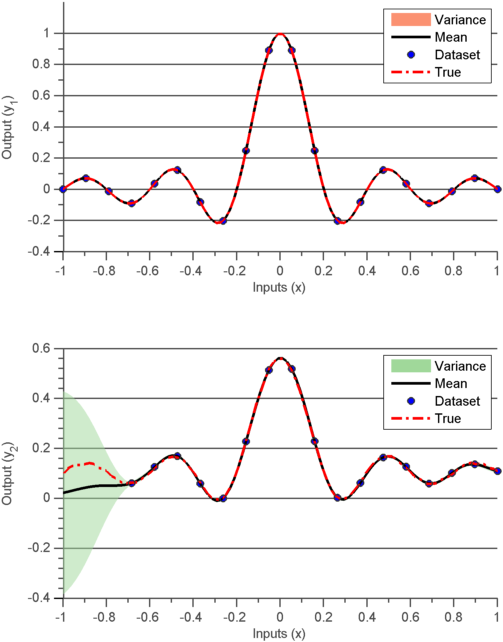
\includegraphics[width=0.29\textwidth]
        {images/part3/independentFitToyData}
        \label{subFigindependentFitToyData}
  }\quad
\subfigure[{GP posterior for a \textbf{simple multi-task} kernel conditioned on the data $\mathcal{D}_{4}$, we choose a SE kernel as the covariance across input points ($k_{inputs} = k_{SE}$). The points where data is unavailable has high value of variance but a better mean prediction when compared to figure \ref{subFigindependentFitToyData}}]
  {
        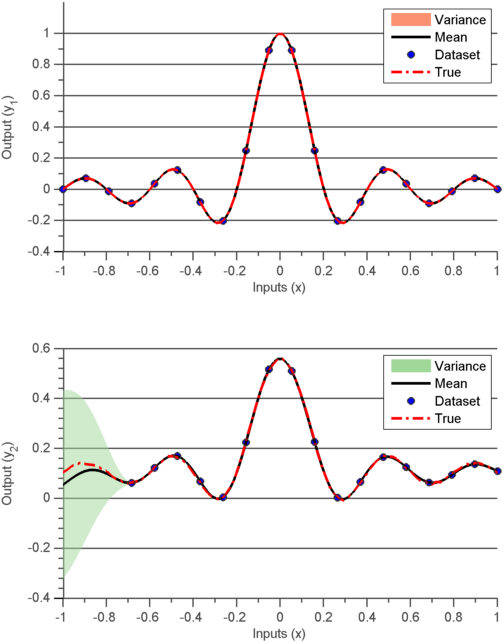
\includegraphics[width=0.29\textwidth]
        {images/part3/multiTaskFitToyData}
        \label{subFigmultiTaskFitToyData}
  }\quad
  \subfigure[{GP posterior for a \textbf{multi-fidelity} kernel conditioned on the data $\mathcal{D}_{4}$. We choose a SE kernel as the covariance across input points ($k_{inputs} = k_{SE}$) and covariance for $\delta$ process, the value of $r(x)$ is kept constant. We can observe that, the prediction at missing points is exact.}]
  {
        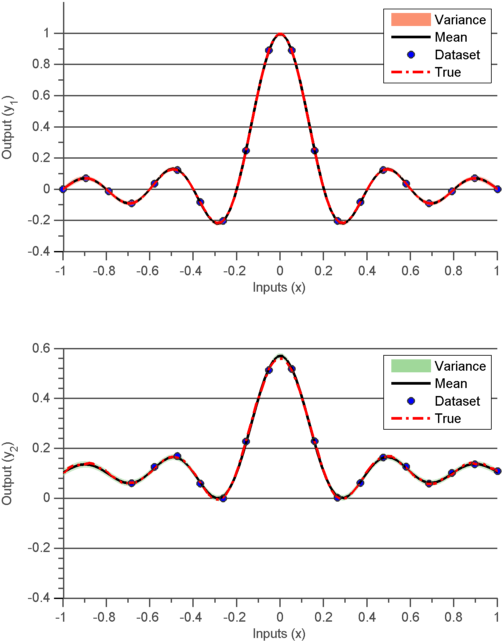
\includegraphics[width=0.29\textwidth]
        {images/part3/multiFidelityFitToyData}
        \label{subFigmultiFidelityFitToyData}
  }\quad

       \caption{Joint Posterior distribution for two outputs with missing data at $x^2 = [-1:-0.75]$. The solid black line defines the mean function, shaded region defines 95\% confidence interval (2$\sigma$) distance away from the mean.}
       \label{figJointPosteriorDistribution}
\end{figure}

\begin{mdframed}[hidealllines=true,backgroundcolor=lightgray!20]
We now compare the accuracy of the three methods but for increasing number of input points. To measure accuracy of the prediction, we again use the the 10-fold Cross Validation (CV). The dataset is divided into 10 subsets, 9 subsets are used to define the training dataset, while the remaining dataset is used to define the test dataset. A model is learned using the training dataset and predictions are performed on the input points of the test dataset. We then calculate the RMSE between the predictions the model and hidden test dataset. This process is repeated 10 times, each time with a different test dataset.  

Figure \ref{subFigboxPlotsToyDataJoint} shows the accuracy of the three methods with increasing number of data-points. The box-plots in red are cases when outputs are assumed independent, the box-plots in green are cases when covariance is assumed to be multi-task, and the box-plots in green are cases when the output covariance is assumed to be multi-fidelity. The error improves with increasing data-points, the multi-fidelity covariance is best for for all the three cases.
\end{mdframed}

\begin{figure}[!ht]
  \centering
    
        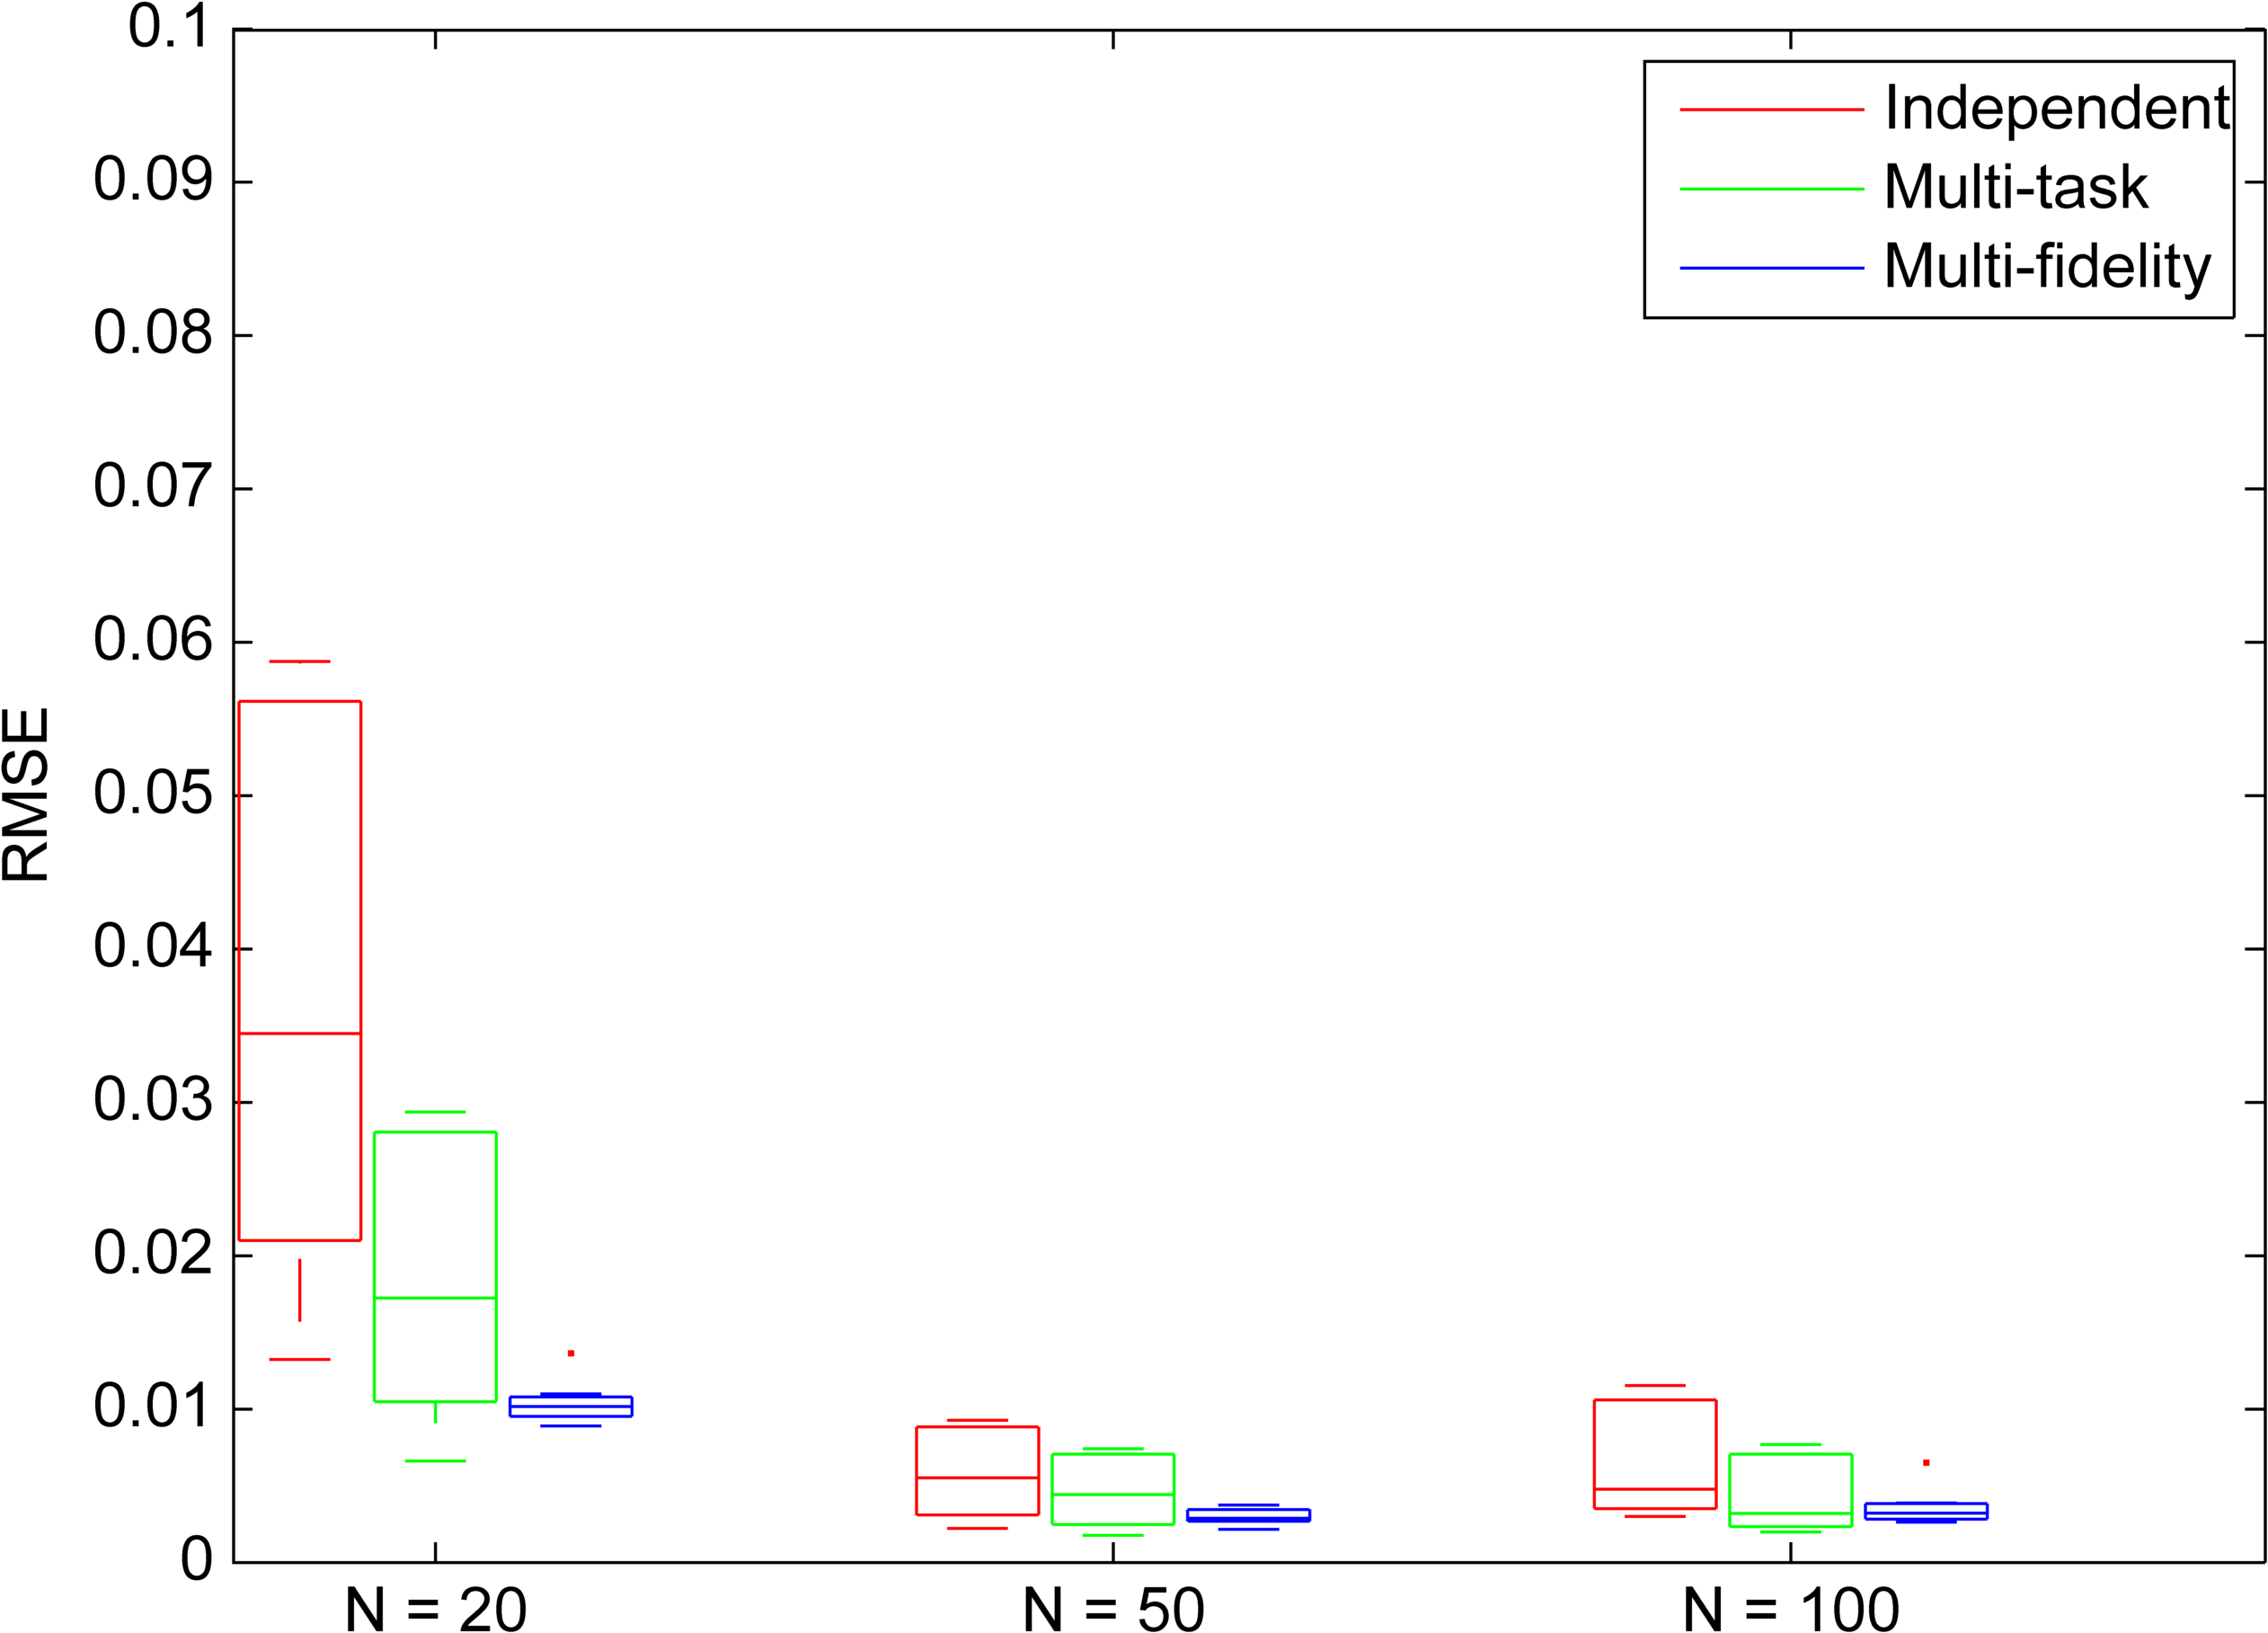
\includegraphics[width=0.45\textwidth]
        {images/part3/boxPlotsToyDataProgressionOverTime}
        \caption{10-fold RMSE box-plots for increasing number of input points. The box-plots in red are cases when outputs are assumed independent, the box-plots in green are cases when covariance is assumed to be multi-task, and the box-plots in green are cases when the output covariance is assumed to be multi-fidelity. The error improves with increasing data-points,the multi-fidelity covariance is best fir for all the three cases.}
        \label{subFigboxPlotsToyDataJoint}
\end{figure}

Multi-fidelity covariance model works so efficiently because the formulation of the second output, the second output is a combination of a multiplication term to the first output $\textcolor{blue}{f^2/2}$ and a new term $\textcolor{red}{0.1cos(f^{1}(x))}$. This is exactly matching the assumptions in the multi-fidelity covariance function. The independent assumption cannot learn the relationship between the outputs, while the multi-task covariance cannot effectively capture the new term $\textcolor{red}{0.1cos(f^{1}(x))}$.

\section{Multi-task for Certification}\label{subsecMTGPExtrapolation}
In this section, we would like to concentrate on the flight-test phase of the aircraft. The goal of an aircraft designer during the flight test phase, is to prove to the certification authorities that the loads predicted during the design cycle phase of the aircraft are equal to the loads experienced by the aircraft during the flight-test phase. Unfortunately, an aircraft manufacturer has access to only a few of test aircrafts during the flight test phase, and each flight-test campaign costing millions of euros. 

This again brings us into the multi-fidelity case, we have access to a relatively simulation model produced during the design phase, and the results of flight-test experiments produced during the certification phase. The results of the simulation model should match the results of the flight-test model. This is not always true, since during simulation the assumptions and inability to model every detail come into play. To resolve this issue the engineering team performs model updating, individual parameters in the simulation model are fine-tuned so as to `update' the simulation model, bringing it as close to the flight test results. The updated model can then be used as a replacement to flight-tests and be used to perform extrapolations in the limit loads conditions.

We wish to replace this model updating phase with a cokriging model. Using the multi-task and multi-fidelity formulation described in chapter \ref{secMTGP} we can encode the simulation model as a prior information. This helps in providing the correct bias and using the years of hard work encoded into the simulation model as a benchmark for learning. 

\textbf{we are tackling experiments hence the noise is not zero}
\textbf{we are also tackling lagged data and hence we will use the delta deflection in the model}

\begin{enumerate}
\item Model update the simulation model
\item Create a surrogate model using flight test experiments, learn pattern automatically
\item Use the simulation model as mean function and learn the difference between the two and learn the pattern automatically
\item Use multi-fidelity modelling 
\item Use multi-fidelity modelling but with noise and time-lag
\end{enumerate}

\subsection{Experiments}

\paragraph{Toy-dataset}

\paragraph{}
The multi-task GP methods introduced in this chapter are pretty common in the literature. The main contribution of this chapter comes in section \ref{}, where we propose a method to extrapolation of high-fidelity data using low-fidelity simulations. These situations are common in an aircraft design cycle during the certification phase. During the certification phase an aircraft manufacturer has access to only a couple of test aircrafts. The main goal of certification is to demonstrate that the loads predicted during detailed design phase are matching during the certification phase. More importantly these loads should be maching or less than the prescribed ones during the limit cases. 
\textbf{Often this is not the case and hence they perform model updating.}
\textbf{We propose to leverage the information of simulations to perform this exrapolation}


Show that co-kriging fails in extrapolation


\section{Discussion}